\documentclass[../main.tex]{subfiles}

\begin{document}
	\section{Sound}
	\begin{preamb}
		Sound is transferred in a form of a wave. In this chapter we will explore the different properties of sound and some of its applications.
	\end{preamb}	
	\subsection{Fundamentals}
	Some fundamental properties of sound:
	\begin{itemize}
		\item Sound is produced by a vibrating source.
		\item Sound exists in the form of a longitudinal wave.
		\item In different media, sound has different speeds. Generally, the higher the density, the faster the speed of sound.
	\end{itemize}
	\begin{center}
		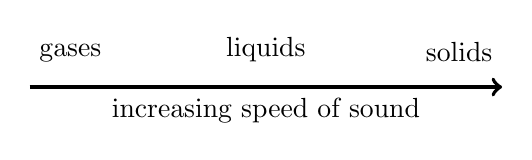
\begin{tikzpicture}
			\draw [line width=0.5mm, ->] (-3,0) -- (3,0) node[anchor=north, pos=0.5 ] {increasing speed of sound};
			\node [anchor=south west] at (-3,0.2) {gases};
			\node [anchor=south] at (0,0.2) {liquids};
			\node [anchor=south east] at (3,0.2) {solids};
		\end{tikzpicture}
	\end{center}
	\peqn{Speed of Sound}{For a sound source from \(d\) away from an observer and capturing it after a time \(t\), the speed of sound can be calculated as}{v = \frac{s}{t}}

\end{document}
